%!TEX root = ../thesis-main.tex

\chapter{Introduzione}\label{chap:introduction}
Il mondo del software ha scritto diverse decadi di storia. Sin dagli anni '50, quando i primi calcolatori programmabili hanno fatto il loro ingresso sul mercato, il software ha assunto un ruolo sempre più pervasivo nella vita quotidiana delle persone. Oltre ad essere parte integrante dei sistemi informativi delle aziende, lo possiamo trovare anche all'interno di automobili, elettrodomestici e tantissimi strumenti con la quale abbiamo a che fare nella nostra quotidianità. La crescente diffusione del software ha introdotto la necessità di progettare metodologie di sviluppo solide e versatili. Uno dei primi è il \textbf{modello a cascata} il quale struttura il processo di realizzazione del software in fasi sequenziali lineari. Il modello riprende la tipica organizzazione della produzione manifatturiera e fu progressivamente abbandonato con l'evolversi delle richieste del mercato. Successivamente prese piede il concetto di modelli iterativi come il \textbf{modello a spirale} in cui il processo di sviluppo è suddiviso in fasi multiple ripetute più volte (iterazioni). Gli ultimi decenni hanno dato vita a un nuovo modello, considerato lo standard dell'industria, la \textbf{metodologia agile}. Quest'ultima non rappresenta un unico modello, ma un insieme di modelli iterativi costruiti sulla base dei principi definiti all'interno del manifesto agile. Questi principi mettono in primo piano un ambiente autonomo e dinamico in cui sono fondamentali: cicli di sviluppo brevi, continui miglioramenti, la comunicazione col cliente e la consegna tempestiva di funzionalità. Il progetto esposto in questo documento introduce un evoluzione del concetto agile nato recentemente nel mondo dello sviluppo del software, conosciuto come ``DevOps".

\section{Contesto}
Con l'avvento di Internet il concetto di software come un entità sviluppata e finita ha completamente cessato di esistere. Mediante la rete è diventato semplice ed efficiente distribuire un programma e fornire un ulteriore supporto attraverso aggiornamenti evolutivi e correttivi. Il fenomeno è cresciuto tanto da aver dato luce alla pratica del rilascio di applicazioni deliberatamente non complete, le quali attraverso il feedback degli utenti evolvono verso un prodotto finito. Il manifesto agile ha introdotto la cultura di emettere frequenti rilasci di nuove versioni del software, rendendo la distribuzione un punto cardine all'interno del ciclo di vita di esso. Dietro lo sviluppo rapido di nuove funzionalità è necessario il rilascio di queste altrettanto velocemente, la filosofia DevOps nasce per soddisfare questa esigenza.

\subsection{DevOps}
La filosofia DevOps (termine nato dalla contrazione di ``Development" ed ``Operations") si è formata intorno al 2008 con l'idea chiave di unire il team di sviluppo ed il team operativo. Il principale catalizzatore di questo concetto è stata la necessità di affrontare inefficienze nelle fasi del ciclo di vita del software. Differentemente dalla metodologia agile, DevOps è una filosofia di sviluppo software che esprime attraverso tre pilastri il suo obiettivo:

\begin{itemize}
	\item il \textbf{flusso}, il miglioramento del flusso di lavoro lungo l'intero processo di produzione, ciò significa ottimizzare il processo dall'idea fino alla generazione di valore con il software in produzione.
	\item Il \textbf{feedback}, mediante cicli di feedback rapidi si garantisce la scoperta di difetti nel codice nelle fasi iniziali del ciclo di vita del prodotto. Ciò comporta rapide correzioni, minor debito tecnico e la garanzia di possedere in qualsiasi momento un software stabile e qualitativamente pronto ad un rilascio.
	\item L'\textbf{apprendimento continuo}, la filosofia DevOps promuove la sperimentazione continua, ossia interrogarsi regolarmente sui possibili miglioramenti attuabili assumendosi i rischi che l'applicazione di questi può recare.
\end{itemize}

Le nozioni fornite dalla cultura DevOps ricoprono diversi ambiti e non si limitano agli aspetti tecnici del ciclo di vita del software. Nella pratica esistono diverse tecnologie che concorrono allo sviluppo di processi conformi alla filosofia presentata.

\begin{figure}[htb]
	\centering
	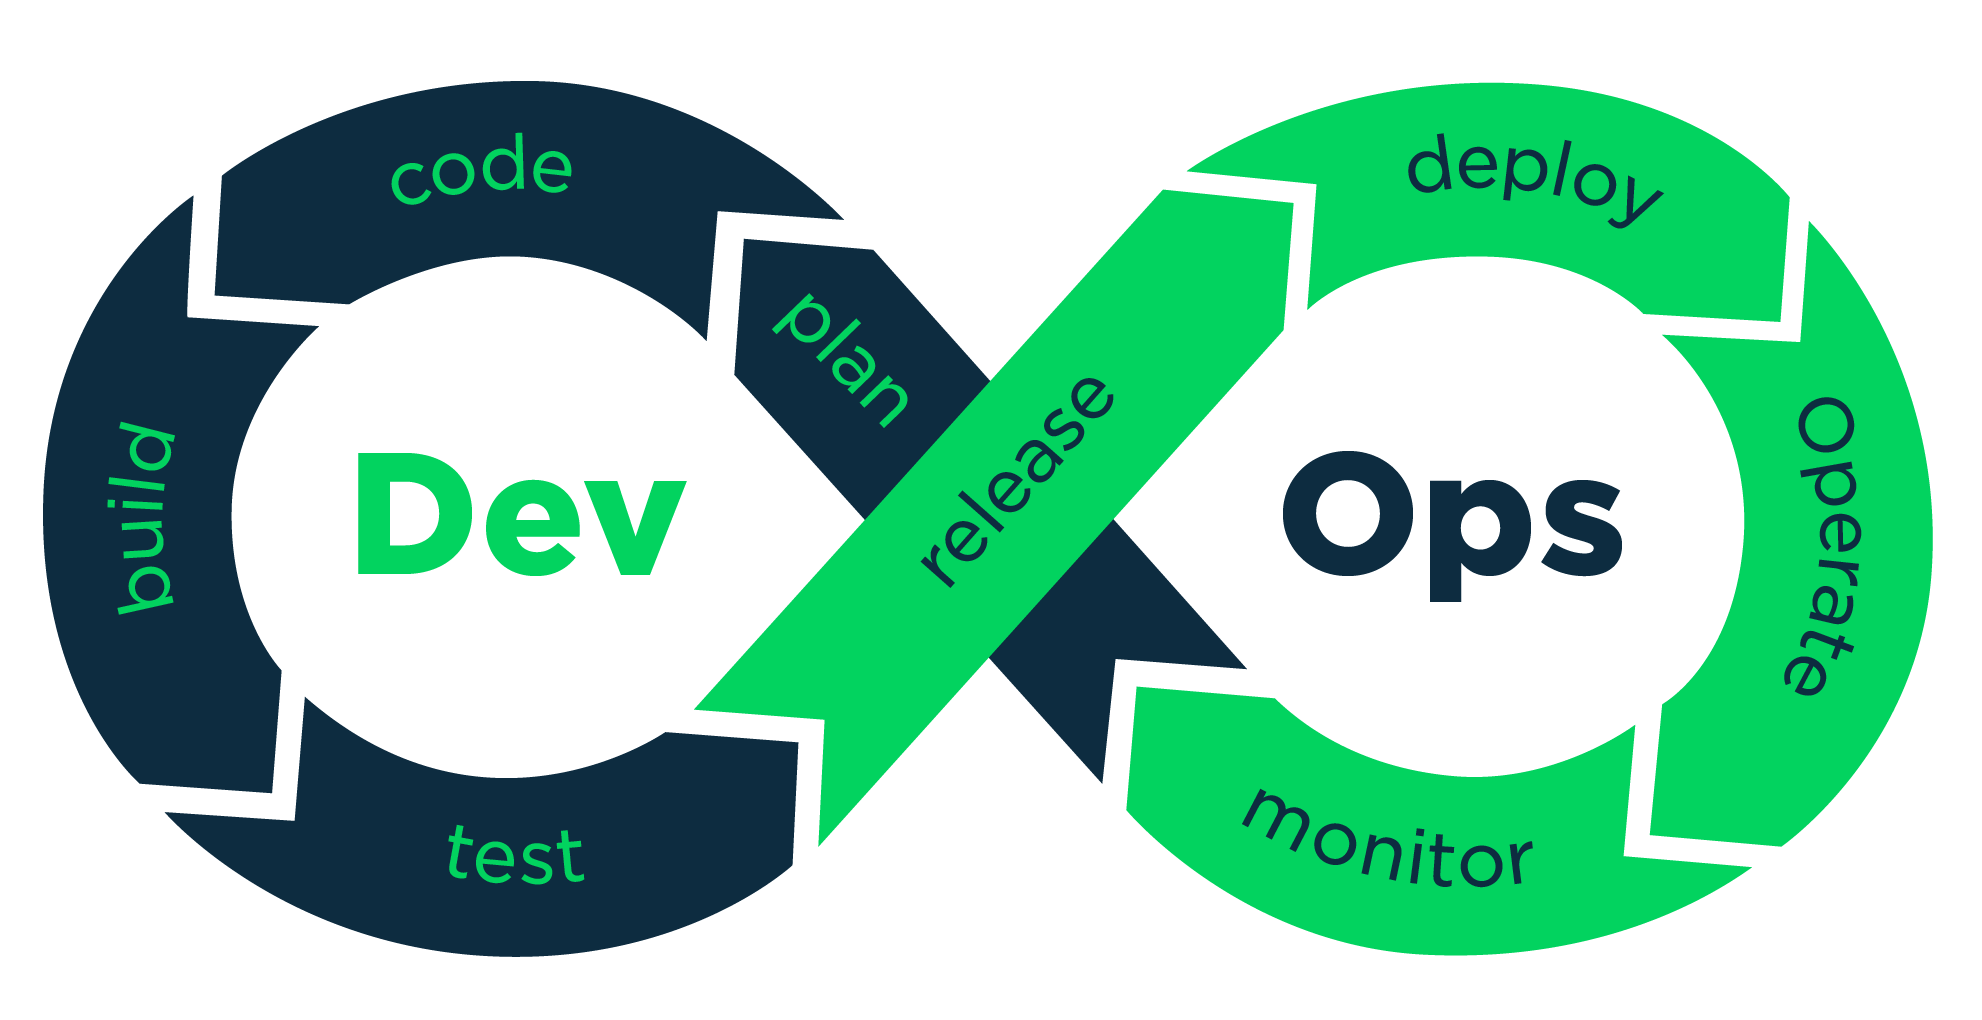
\includegraphics[width=.8\linewidth]{figures/devops-process.png}
	\caption{Le fasi della metodologia DevOps}
	\label{fig:devops-process}
\end{figure}

Il modello illustrato nella figura \ref{fig:devops-process} rappresenta il ciclo di vita del software secondo la filosofia DevOps. La disposizione delle fasi, configurata in modo da evocare il simbolo dell'infinito, simboleggia il concetto di continuità fondamentale per questa filosofia. Questo concetto è introdotto all'interno del flusso mediante un altro pilastro: l'\textit{automazione}. Grazie all'automazione, gli sviluppatori possono delegare compiti complessi o ripetitivi a sistemi esterni configurando tre componenti chiave: un evento, un'azione e il risultato atteso. Quando si verifica un evento specifico, un'entità esterna esegue un insieme di azioni predeterminate, il cui successo o fallimento viene determinato dal confronto con il risultato atteso. A livello pratico, ciò è ottenuto mediante l'utilizzo di server o più generalmente infrastrutture cloud complesse.

L'automazione dunque garantisce l'esecuzione dei processi in modo consistente e permette di concentrare le risorse del team sullo sviluppo, eliminando quindi l'intervento umano da compiti ripetitivi e passibili di errori. Una delle pratiche più diffuse, concetto rilevante della filosofia DevOps, è la costruzione di una pipeline di \ac{cicd}.

\paragraph{Continuous integration} La pratica della \textit{continuous integration} si concentra sull'integrazione automatica e continua delle modifiche al codice sorgente del progetto. Tipicamente, il processo si articola nei seguenti passaggi: (i) gli sviluppatori introducono nuovo codice nel progetto attraverso il software di \textit{version control}, (ii) un server acquisisce le modifiche, compila e testa l'intero progetto, (iii) una volta completato il processo, comunica agli sviluppatori l'esito delle operazioni. Questo approccio consente di individuare errori nel codice anticipatamente, garantendo stabilità e una maggiore qualità al software.

Un aspetto fondamentale è la stesura dei test: un'eccessiva copertura può rallentare il processo di integrazione. È pertanto essenziale bilanciare la copertura dei test in base alle esigenze del progetto, tenendo presente che un aumento della copertura riduce il rischio di introdurre codice difettoso.

\paragraph{Continuous delivery} La distribuzione rappresenta l'insieme di operazioni finalizzate alla consegna del software agli utenti finali. Questo processo estende l'integrazione continua e si preoccupa di garantire la disponibilità costante di un artefatto di build pronto per il rilascio. L'effettivo rilascio di una nuova versione del software può avvenire in modo automatico oppure manualmente da parte dello sviluppatore. La filosofia DevOps fornisce linee guida e non regole rigide, lasciando al team di sviluppo il compito di progettare ed integrare un flusso adeguato alle necessità del progetto.

\subsection{Software JVM-based}
Per ``software JVM-based" si intendono i programmi e le applicazioni realizzate mediante linguaggi di programmazione eseguiti e compilati per la \ac{jvm}. Introdotta nel 1995, la Java Virtual Machine ha rivoluzionato il mondo dello sviluppo del software introducendo un nuovo livello di astrazione nella compilazione ed esecuzione dei programmi. Il linguaggio Java, sviluppato appositamente per l'omonima macchina virtuale, è un linguaggio di programmazione ad alto livello orientato agli oggetti progettato per avere il minor numero di dipendenze esterne possibile, in modo da garantire la sua portabilità. L'esecuzione di un programma Java (\cref{fig:java-execution}) avviene per fasi differenti rispetto ad un normale linguaggio compilato: il codice viene tradotto, in una prima fase di compilazione, in \textit{bytecode}, un linguaggio intermedio. Quest'ultimo è successivamente fornito alla macchina virtuale, la quale interpreta il bytecode generato e lo traduce in codice macchina del sistema sottostante.

\imagesource{figures/java-program-execution.png}{https://commons.wikimedia.org/wiki/File:Java-program-execution.png}{Il processo di compilazione di un programma Java e la sua esecuzione mediante una \ac{jvm}}{.6}{java-execution}

Inizialmente progettata per ospitare il linguaggio Java, nel corso del tempo la \ac{jvm} ha visto l'adozione di diversi altri linguaggi di programmazione e l'adattamento di alcuni provenienti da ambienti diversi. Il suo impatto nel mondo del software fu ed è ancora attualmente rilevante, tanto che due indici di valutazione della popolarità dei linguaggi di programmazione posizionano i due principali linguaggi \ac{jvm} all'interno della top 20, con Java, il più datato, nella top 5 (TIOBE\footnote{https://www.tiobe.com/tiobe-index/} e PYPL\footnote{https://pypl.github.io/PYPL.html} index). Una delle caratteristiche che ha decretato il successo di questa architettura è la portabilità. L'integrazione di un linguaggio intermedio permette di astrarre dalla piattaforma di esecuzione, consentendo, mediante un singolo codice sorgente, di distribuire l'applicativo su differenti sistemi operativi con persino architetture hardware diverse.

Un aspetto cruciale nel rilascio di un'applicazione è la sua distribuzione. La forma e il metodo adottati devono garantire un processo di installazione scorrevole, privo di intoppi e consistente, in modo che gli utenti possano installare l'applicativo nel proprio sistema senza preoccuparsi di dipendenze esterne. Tuttavia, questa necessità presenta sfide specifiche nell'ambito dei linguaggi di programmazione interpretati, come quelli \ac{jvm}-based.

\subsection{Problematiche della pacchettizzazione}
Con il termine ``pacchettizzazione" si intende il processo di creazione di un singolo file, comunemente chiamato \textit{archivio}, che contiene l'applicazione e le risorse necessarie alla sua esecuzione. Nell'ambito dei linguaggi compilati, questo viene realizzato distribuendo archivi che contengono file eseguibili in codice macchina e le librerie dinamiche necessarie all'esecuzione dell'applicativo.

L'esecuzione di un programma Java richiede inevitabilmente la presenza di una \ac{jvm}, o più precisamente un \ac{jre}. Generalmente, i software realizzati con linguaggi basati su JVM vengono distribuiti attraverso due diverse tipologie di file:
\begin{itemize}
	\item un archivio \textbf{JAR} (\textit{java archive}), un file archivio contenente i \textit{classfiles}, ovvero il bytecode interpretato dalla \ac{jvm} necessario per eseguire l'applicazione;
	\item oppure un archivio \textbf{WAR} (\textit{web application resource}), il quale è simile al Jar, ma è utilizzato più specificatamente per la distribuzione di applicazioni web realizzate con Java.
\end{itemize}
Come già evidenziato, i due archivi differiscono dalle controparti dei linguaggi compilati poiché richiedono la presenza di un ambiente Java globale sul dispositivo in cui viene eseguito l'applicativo. Questo comporta un passo indietro rispetto ai principi della distribuzione del software, in quanto introduce una dipendenza esterna con cui l'utente è costretto a confrontarsi. La distribuzione ottimale di un software \ac{jvm} richiede quindi un approccio differente rispetto alle normali applicazioni compilate.

\subsection{Package manager}

Nell'ambito della distribuzione è importante considerare il ruolo dei \textit{package manager} nei sistemi operativi odierni. Il \textit{package management system} è un insieme di strumenti software che gestiscono i processi di installazione, aggiornamento, configurazione e rimozione di applicativi dal sistema. Esso opera attraverso tre componenti principali:
\begin{itemize}
	\item un componente a basso livello, che si occupa principalmente dell'installazione o rimozione dei pacchetti;
	\item un componente ad alto livello, il cui compito principale è quello di fornire un'interfaccia all'utente e di risolvere le dipendenze;
	\item i repository, ossia archivi pubblici online dalla quale l'interfaccia ad alto livello ottiene i pacchetti e i relativi meta-dati.
\end{itemize}
\begin{figure}[htb]
	\centering
	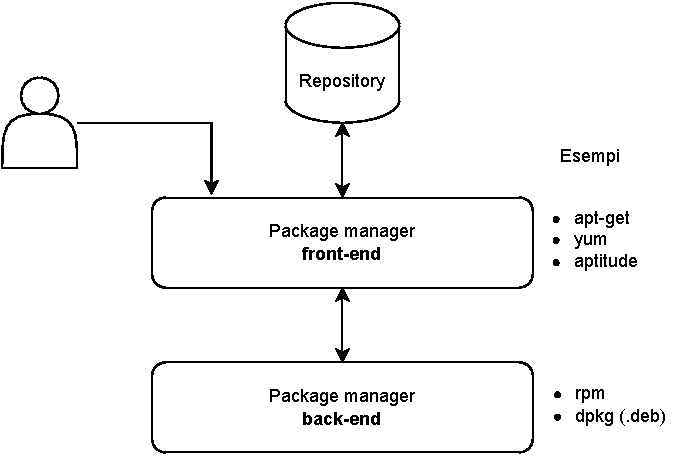
\includegraphics[width=.7\linewidth]{figures/package-managers.pdf}
	\caption{Struttura più diffusa dei sistemi di gestione di pacchetti}
	\label{fig:package-managers}
\end{figure}
L'utilizzo dei package manager (\cref{fig:package-managers}) fornisce diversi vantaggi nella gestione di un sistema: (i) semplifica notevolmente il processo di aggiornamento, in quanto mediante un comando è possibile aggiornare tutti i componenti, ed allo stesso tempo, (ii) funziona da strumento di installazione capace di reperire pacchetti distribuiti in archivi online ed installarli nel sistema. I vantaggi descritti hanno contribuito a una loro notevole diffusione, in maggior parte tra gli utenti avanzati per via dell'utilizzo della \ac{cli} che molti di questi fanno. Tuttavia, nei sistemi operativi Linux, dove il package manager è essenziale e pervasivo, molte distribuzioni forniscono in aggiunta interfacce grafiche progettate appositamente per l'uso da parte di utenti meno esperti.

In conclusione, i software \ac{jvm}-based sono ampiamente diffusi nel mercato e gran parte della loro popolarità deriva dalle loro caratteristiche, come la portabilità. Tuttavia, nonostante siano eseguibili su qualsiasi sistema operativo, la loro distribuzione non è semplice. Se le problematiche evidenziate si riferiscono principalmente alla forma, i package manager in contrasto offrono, mediante i repository online, un processo di distribuzione solido e funzionale.

\section{Motivazioni e Obiettivi}
I punti discussi precedentemente hanno evidenziato l'importanza che l'automazione ricopre all'interno dello sviluppo del software. Il rilascio continuo di un applicazione è necessario per mantenere elevati standard di qualità e comporta la necessità di automatizzare questi processi per garantire la loro esecuzione in modo consistente. 

Il rilascio di un'applicazione coinvolge due importanti fattori: (i) la forma, il file consegnato all'utente intenzionato ad installare il software e (ii) il processo, le modalità con cui l'utente ottiene il file adibito all'installazione. Nel contesto dei software \ac{jvm}, la loro forma di distribuzione solleva problematiche legate alla natura dei linguaggi interpretati, perciò richiedono uno studio approfondito al fine di garantire un sistema di installazione funzionale e consistente. Contemporaneamente i sistemi di gestione dei pacchetti, sono candidati ideali per garantire un processo di distribuzione solido all'interno del vasto panorama dei sistemi operativi più diffusi.

\subsection{Obiettivi}

L'obiettivo principale dell'elaborato è quindi quello di progettare un sistema di pacchettizzazione e distribuzione automatica di un software \ac{jvm} all'interno di una pipeline di integrazione e distribuzione continua. I processi si occupano di pacchettizzare e dunque produrre un archivio di installazione conforme e valido in modo automatico nel momento in cui una nuova versione del software viene rilasciata, inoltre, provvedono a distribuire questi nei repository pubblici di riferimento di package manager selezionati, in modo da eliminare totalmente l'intervento umano nel processo di rilascio dell'applicazione. Ambedue i processi devono prevedere l'esecuzione di test all'interno del flusso di distribuzione, in tal modo si garantisce un feedback immediato nell'eventualità che gli artefatti o i processi di pubblicazione siano difettosi.
\begin{figure}[htb]
	\centering
	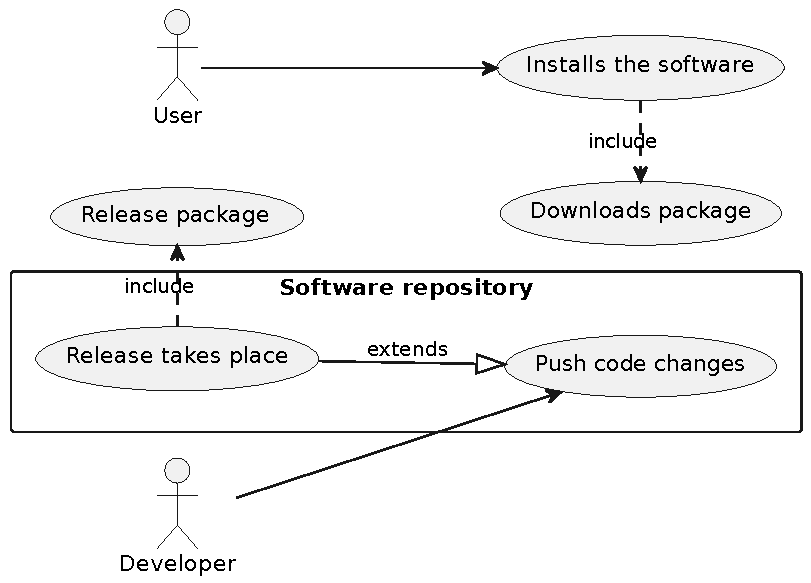
\includegraphics[width=.75\linewidth]{figures/use-case-diagram.pdf}
	\caption{Diagramma dei casi d'uso dallo sviluppatore all'utente}
	\label{fig:use-case-diagram}
\end{figure}
Nella \Cref{fig:use-case-diagram} sono rappresentati gli scenari di utilizzo da parte degli utenti finali e degli sviluppatori. In particolare, lo sviluppatore introduce nuovo codice all'interno del repository del progetto e successivamente l'esecuzione della pipeline determina se è necessario il rilascio di una nuova versione. In caso di esito positivo, i pacchetti di installazione sono generati. Questi, una volta distribuiti, consentiranno agli utenti di introdurre il software nel proprio sistema.